\chapter{Vector calculus}


\section{Gradient of real-valued multivariate functions}

\begin{description}
    \item[Gradient] \marginnote{Gradient}
        Given a function $f: \mathbb{R}^n \rightarrow \mathbb{R}$, 
        the gradient is a row vector containing the partial derivatives of $f$:
        \[ 
            \nabla f(\vec{x}) = 
            \begin{pmatrix}
                \frac{\partial f(\vec{x})}{\partial x_1} & \frac{\partial f(\vec{x})}{\partial x_2} & \dots & \frac{\partial f(\vec{x})}{\partial x_n}
            \end{pmatrix}
            \in \mathbb{R}^{1 \times n}
        \]

    \item[Hessian] \marginnote{Hessian matrix}
        Given a function $f: \mathbb{R}^n \rightarrow \mathbb{R}$, 
        the Hessian matrix $\matr{H} \in \mathbb{R}^{n \times n}$ contains the second derivatives of $f$:
        \[
            \matr{H} = 
            \begin{pmatrix}
                \frac{\partial f}{\partial x_1^2}               & \frac{\partial f}{\partial x_1 \partial x_2} & \dots & \frac{\partial f}{\partial x_1 \partial x_n} \\
                \frac{\partial f}{\partial x_2 \partial x_1}    & \frac{\partial f}{\partial x_2^2} & \dots & \vdots \\
                \vdots                                          & \vdots & \ddots & \vdots \\
                \frac{\partial f}{\partial x_n \partial x_1}    & \dots & \dots & \frac{\partial f}{\partial x_n^2}
            \end{pmatrix} 
        \]
        In other words, $H_{i,j} = \frac{\partial f}{\partial x_i \partial x_j}$.
        Moreover, $\matr{H}$ is symmetric.
\end{description}

\subsection{Partial differentiation rules}
\begin{description}
    \item[Product rule] \marginnote{Product rule}
        Let $f, g: \mathbb{R}^n \rightarrow \mathbb{R}$:
        \[ 
            \frac{\partial}{\partial \vec{x}} (f(\vec{x})g(\vec{x})) = 
                \frac{\partial f}{\partial \vec{x}} g(\vec{x}) + f(\vec{x}) \frac{\partial g}{\partial \vec{x}}
        \]
    \item[Sum rule] \marginnote{Sum rule}
        Let $f, g: \mathbb{R}^n \rightarrow \mathbb{R}$:
        \[
            \frac{\partial}{\partial \vec{x}} (f(\vec{x}) + g(\vec{x})) =
                \frac{\partial f}{\partial \vec{x}} + \frac{\partial g}{\partial \vec{x}}
        \]
    \item[Chain rule] \marginnote{Chain rule}
        Let $f: \mathbb{R}^n \rightarrow \mathbb{R}$ and $\vec{g}$ a vector of $n$ functions $g_i: \mathbb{R}^m \rightarrow \mathbb{R}$:
        \[
            \frac{\partial}{\partial \vec{x}} (f \circ \vec{g})(\vec{x}) = 
                \frac{\partial}{\partial \vec{x}} \Big( f(\vec{g}(\vec{x})) \Big) =
                \frac{\partial f}{\partial \vec{g}} \frac{\partial \vec{g}}{\partial \vec{x}}
        \]

        For instance, consider a $f: \mathbb{R}^2 \rightarrow \mathbb{R}$ of two variables 
        $g_1(t), g_2(t): \mathbb{R} \rightarrow \mathbb{R}$ that are functions of $t$. 
        The gradient of $f$ with respect to $t$ is:
        \[
            \frac{\text{d}f}{\text{d}t} = 
            % \frac{\partial f}{\partial (g_1, g_2)} \frac{\partial (g_1, g_2)}{\partial t} =
            \begin{pmatrix}
                \frac{\partial f}{\partial g_1} & \frac{\partial f}{\partial g_2}
            \end{pmatrix}
            \begin{pmatrix}
                \frac{\partial g_1}{\partial t} \\ \frac{\partial g_2}{\partial t}
            \end{pmatrix}
            = \frac{\partial f}{\partial g_1} \frac{\partial g_1}{\partial t} + \frac{\partial f}{\partial g_2} \frac{\partial g_2}{\partial t}
        \]
        In other words, the first matrix represents the gradient of $f$ w.r.t. its variables and 
        the second matrix contains in the $i$-th row the gradient of $g_i$.

        Therefore, if $g_i$ are in turn multivariate functions $g_1(s, t), g_2(s, t): \mathbb{R}^2 \rightarrow \mathbb{R}$,
        the chain rule can be applied as follows:
        \[
            \frac{\text{d}f}{\text{d}(s, t)} = 
            \begin{pmatrix}
                \frac{\partial f}{\partial g_1} & \frac{\partial f}{\partial g_2}
            \end{pmatrix}
            \begin{pmatrix}
                \frac{\partial g_1}{\partial s} & \frac{\partial g_1}{\partial t} \\ 
                \frac{\partial g_2}{\partial s} & \frac{\partial g_2}{\partial t}
            \end{pmatrix}
        \]

        \begin{example}
            Let $f(x_1, x_2) = x_1^2 + 2x_2$, where $x_1 = \sin(t)$ and $x_2 = \cos(t)$.
            \[
                \begin{split}
                    \frac{\text{d}f}{\text{d}t} & = 
                        \frac{\partial f}{\partial x_1}\frac{\partial x_1}{\partial t} + \frac{\partial f}{\partial x_2}\frac{\partial x_2}{\partial t} \\
                        & = (2x_1)(\cos(t)) + (2)(-\sin(t)) \\
                        & = 2\sin(t)\cos(t) - 2\sin(t)
                \end{split}
            \]
        \end{example}

        \begin{example}
            Let $h: \mathbb{R} \rightarrow \mathbb{R}$ be defined as $h(t) = (f \circ \vec{g})(t) = f(\vec{g}(t))$ where:
            \[ f: \mathbb{R}^2 \rightarrow \mathbb{R} \text{ is defined as } f(g_1, g_2) = \exp(g_1 g_2^2) \]
            \[ 
                \vec{g}: \mathbb{R} \rightarrow \mathbb{R}^2 \text{ is defined as } 
                \vec{g}(t) = \begin{pmatrix} g_1 \\ g_2 \end{pmatrix} = \begin{pmatrix}t \cos(t) \\ t \sin(t) \end{pmatrix}
            \]
            The gradient of $h$ with respect to $t$ can be computed as:
            \[
                \frac{\text{d} h}{\text{d} t} =
                    \frac{\partial f}{\partial \vec{g}} \frac{\partial \vec{g}}{\partial t} =
                    \begin{pmatrix}
                        \frac{\partial f}{\partial g_1} & \frac{\partial f}{\partial g_2}
                    \end{pmatrix}
                    \begin{pmatrix}
                        \frac{\partial g_1}{\partial t} \\ \frac{\partial g_2}{\partial t}
                    \end{pmatrix}
            \]
            \[
                = 
                \begin{pmatrix} \exp(g_1 g_2^2)g_2^2 & 2\exp(g_1 g_2^2)g_1 g_2 \end{pmatrix}
                \begin{pmatrix} \cos(t) + (-t\sin(t)) \\ \sin(t) + t\cos(t) \end{pmatrix}
            \]
        \end{example}

        \begin{example}[Gradient of a least squares loss] \marginnote{Least squares loss gradient}
            Given a linear model defined on $\vec{\uptheta}$:
            \[ \vec{y} = \matr{\Phi}\vec{\uptheta} \]
        \end{example}
        with $\vec{\uptheta} \in \mathbb{R}^D$, $\matr{\Phi} \in \mathbb{R}^{N \times D}$ and $\vec{y} \in \mathbb{R}^N$.
        We can define the least squares loss function as:
        \[ L(\vec{e}) = \Vert \vec{e} \Vert_2^2 \]
        \[ \vec{e}(\vec{\uptheta}) = \vec{y} - \matr{\Phi}\vec{\uptheta} \]
        It must be noted that:
        \[ L(\vec{e}) = \Vert \vec{e} \Vert_2^2 = \vec{e}^T\vec{e} = \sum_{i=1}^{N} \vec{e}_i^2 \]

        To compute the gradient of $L$ with respect to $\vec{\uptheta}$, we can use the chain rule:
        \[ 
            \begin{split}
                \nabla L(\vec{\uptheta}) &= \frac{\partial L}{\partial \vec{e}} \frac{\partial \vec{e}}{\partial \vec{\uptheta}} 
                        = (2\vec{e}^T) (-\matr{\Phi}) \\
                    & = -2(\vec{y}^T - \vec{\uptheta}^T \matr{\Phi}^T)\matr{\Phi} \\
                    & = -2(\vec{y}^T\matr{\Phi} - \vec{\uptheta}^T \matr{\Phi}^T\matr{\Phi})
            \end{split}
        \]

        Note that if we enforce $\nabla L(\vec{\uptheta}) = \nullvec$, we obtain the normal equation of \Cref{sec:lls}:
        \[
            \begin{split}
                \nabla L = 0 &\iff -2(\vec{y}^T\matr{\Phi} - \vec{\uptheta}^T \matr{\Phi}^T\matr{\Phi}) = \nullvec \\
                    &\iff \vec{y}^T \matr{\Phi} - \vec{\uptheta}^T \matr{\Phi}^T\matr{\Phi} = \nullvec \\
                    &\iff \matr{\Phi}^T \vec{y} - \matr{\Phi}^T \matr{\Phi} \vec{\uptheta} = \nullvec
            \end{split}
        \]
\end{description}



\section{Gradient of vector-valued multivariate functions}

\begin{description}
    \item[Vector-valued function]
        Function $\vec{f}: \mathbb{R}^n \rightarrow \mathbb{R}^m$ with $n \geq 1$ and $m > 1$.
        Given $\vec{x} \in \mathbb{R}^n$, the output can be represented as:
        \[
            \vec{f}(\vec{x}) = 
            \begin{pmatrix}
                f_1(\vec{x}) \\ \vdots \\ f_m(\vec{x})
            \end{pmatrix} \in \mathbb{R}^m
        \]
        where $f_i: \mathbb{R}^n \rightarrow \mathbb{R}$.

    \item[Jacobian] \marginnote{Jacobian matrix}
        Given $\vec{f}: \mathbb{R}^n \rightarrow \mathbb{R}^m$, the Jacobian matrix $\matr{J} \in \mathbb{R}^{m \times n}$
        contains the first-order derivatives of $\vec{f}$:
        \[
            \matr{J} = \nabla\vec{f}(\vec{x}) = 
            \begin{pmatrix}
                \frac{\partial \vec{f}(\vec{x})}{\partial x_1} & \dots & \frac{\partial \vec{f}(\vec{x})}{\partial x_n}
            \end{pmatrix} = 
            \begin{pmatrix}
                \frac{\partial f_1(\vec{x})}{\partial x_1} & \dots & \frac{\partial f_1(\vec{x})}{\partial x_n} \\
                \vdots & \ddots & \vdots \\
                \frac{\partial f_m(\vec{x})}{\partial x_1} & \dots & \frac{\partial f_m(\vec{x})}{\partial x_n} \\
            \end{pmatrix}
        \]
        In other words, $J_{i,j} = \frac{\partial f_i}{\partial x_j}$.
        Note that the Jacobian matrix is a generalization of the gradient in the real-valued case.
    \end{description}



\section{Backpropagation}
\marginnote{Backpropagation}
Backpropagation is used to tune the parameters of a neural network.
A neural network can be seen as a composition of many functions:
\[ \vec{y} = (\vec{f}_K \circ \vec{f}_{K-1} \circ \dots \circ \vec{f}_1)(\vec{x}) = \vec{f}_K(\vec{f}_{K-1}(\cdots \vec{f}_1(\vec{x}) \cdots)) \]
Each $\vec{f}_i$ takes as input the output of the previous layer $\vec{x}_{i-1}$ and has the form:
\[ \vec{f}_i(\vec{x}_{i-1}) = \sigma_i(\matr{A}_{i-1}\vec{x}_{i-1} + \vec{b}_{i-1}) \]
where $\sigma_i$ is an activation function\footnote{\url{https://en.wikipedia.org/wiki/Activation_function}} (a function to add nonlinearity), 
while $\matr{A}_{i-1}$ (linear mapping) and $\vec{b}_{i-1}$ (biases) are the parameters of $\vec{f}_i$.

\begin{figure}[ht]
    \centering
    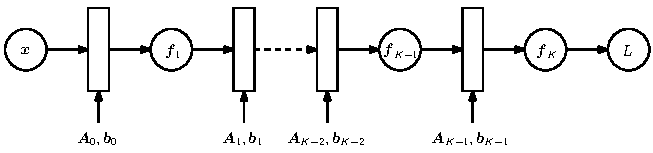
\includegraphics[width=0.7\textwidth]{img/_forward_pass.pdf}
    \caption{Forward pass}
\end{figure}

We can more compactly denote a neural network with input $\vec{x}$ and $K$ layers as:
\[ 
    \begin{split}
        \vec{f}_0 &= \vec{x} \\
        \vec{f}_i &= \sigma_i(\matr{A}_{i-1} \vec{f}_{i-1} + \vec{b}_{i-1}) \text{ } i=1, \dots, K
    \end{split}
\]
Given the ground truth $\vec{y}$, we want to find the parameters $\matr{A}_j$ and $\vec{b}_j$ that minimize the squared loss:
\[ L(\vec{\uptheta}) = \Vert \vec{y} - \vec{f}_K(\vec{\uptheta}, \vec{x}) \Vert^2 \]
where $\vec{\uptheta} = \{ \matr{A}_{0}, \vec{b}_{0}, \dots, \matr{A}_{K-1}, \vec{b}_{K-1} \}$ are the parameters of each layer.
This can be done by using the chain rule to compute the partial derivatives of $L$ with respect to the parameters $\vec{\uptheta}_j = \{ \matr{A}_j, \vec{b}_j \}$:
\[
    \begin{split}
        \frac{\partial L}{\partial \vec{\uptheta}_{K-1}} &= 
            \overbrace{\frac{\partial L}{\partial \vec{f}_K} \frac{\partial \vec{f}_K}{\partial \vec{\uptheta}_{K-1}}}^{\mathclap{\text{New}}} \\
        \frac{\partial L}{\partial \vec{\uptheta}_{K-2}} &= 
            \overbrace{\frac{\partial L}{\partial \vec{f}_K}}^{\mathclap{\text{Known}}}
            \overbrace{\frac{\partial \vec{f}_K}{\partial \vec{f}_{K-1}} \frac{\partial \vec{f}_{K-1}}{\partial \vec{\uptheta}_{K-2}}}^{\mathclap{\text{New}}} \\
        \frac{\partial L}{\partial \vec{\uptheta}_{K-3}} &= 
            \overbrace{\frac{\partial L}{\partial \vec{f}_K} \frac{\partial \vec{f}_K}{\partial \vec{f}_{K-1}}}^{\mathclap{\text{Known}}}
            \overbrace{\frac{\partial \vec{f}_{K-1}}{\partial \vec{f}_{K-2}} \frac{\partial \vec{f}_{K-2}}{\partial \vec{\uptheta}_{K-3}}}^{\mathclap{\text{New}}} \\
        \vdots \\
        \frac{\partial L}{\partial \vec{\uptheta}_{i}} &= 
            \overbrace{\frac{\partial L}{\partial \vec{f}_K} \frac{\partial \vec{f}_K}{\partial \vec{f}_{K-1}} \dots}^{\mathclap{\text{Known}}}
            \overbrace{\frac{\partial \vec{f}_{i+2}}{\partial \vec{f}_{i+1}} \frac{\partial \vec{f}_{i+1}}{\partial \vec{\uptheta}_{i}}}^{\mathclap{\text{New}}}
    \end{split}
\]

\begin{figure}[ht]
    \centering
    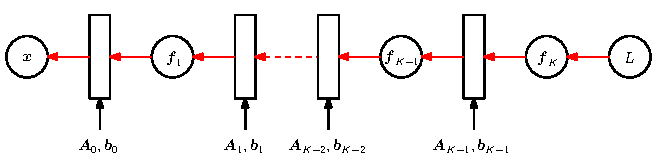
\includegraphics[width=0.7\textwidth]{img/_backward_pass.pdf}
    \caption{Backward pass}
\end{figure}



\section{Automatic differentiation}
Starting from the example below first is recommended.\\

\marginnote{Automatic differentiation}
Automatic differentiation allows to numerically compute 
the gradient of complex functions using elementary functions, intermediate variables and the chain rule through a computation graph.
When the gradient has many components, it also allows to compute it more efficiently.

Let $f$ be a function,
$x_1, \dots, x_d$ the input variables of $f$,
$x_{d+1}, \dots, x_{D-1}$ the intermediate variables and
$x_D$ the output variable.
The computation graph can be expressed as:
\[
    \forall i \in \{ d+1, \dots, D \}: x_i = g_i(x_{\text{Pa}(x_i)})
\]
where $g_i$ are elementary functions and $x_{\text{Pa}(x_i)}$ are the parent nodes of $x_i$ in the graph.
In other words, each intermediate variable is expressed as an elementary function of its preceding nodes.
The derivatives of $f$ can then be computed step-by-step going backward as:
\[ \frac{\partial f}{\partial x_D} = 1 \text{, as by definition } f = x_D \]
\[ 
    \frac{\partial f}{\partial x_i} = \sum_{\forall x_c: x_i \in \text{Pa}(x_c)} \frac{\partial f}{\partial x_c} \frac{\partial x_c}{\partial x_i}
        = \sum_{\forall x_c: x_i \in \text{Pa}(x_c)} \frac{\partial f}{\partial x_c} \frac{\partial g_c}{\partial x_i}
\]
where $\text{Pa}(x_c)$ is the set of parent nodes of $x_c$ in the graph.
In other words, to compute the partial derivative of $f$ w.r.t. $x_i$, 
we apply the chain rule by computing 
the partial derivative of $f$ w.r.t. the variables following $x_i$ in the graph (as the computation goes backward).

Automatic differentiation is applicable to all functions that can be expressed as a computational graph and 
when the elementary functions are differentiable.
Note that backpropagation is a special case of automatic differentiation.

\begin{example}
    Given the function:
    \[ f(x) = \sqrt{x^2 + \exp(x^2)} + \cos(x^2 + \exp(x^2)) \]
    and the elementary functions $\{ (\cdot)^2, \exp(\cdot), +, \sqrt{\cdot}, \cos(\cdot) \}$,
    $f$ can be decomposed in the following intermediate variables:\\
    \begin{minipage}{.5\linewidth}
        \[
            \begin{split}
                a &= x^2        \\
                b &= \exp(a)    \\
                c &= a + b      \\
                d &= \sqrt{c}   \\
            \end{split} 
        \]
    \end{minipage}%
    \begin{minipage}{.5\linewidth}
        \[
            \begin{split}
                e &= \cos(c)    \\
                f &= d + e      \\
            \end{split} 
        \]
    \end{minipage}\\

    Which corresponds to the following computation graph:
    \begin{center}
        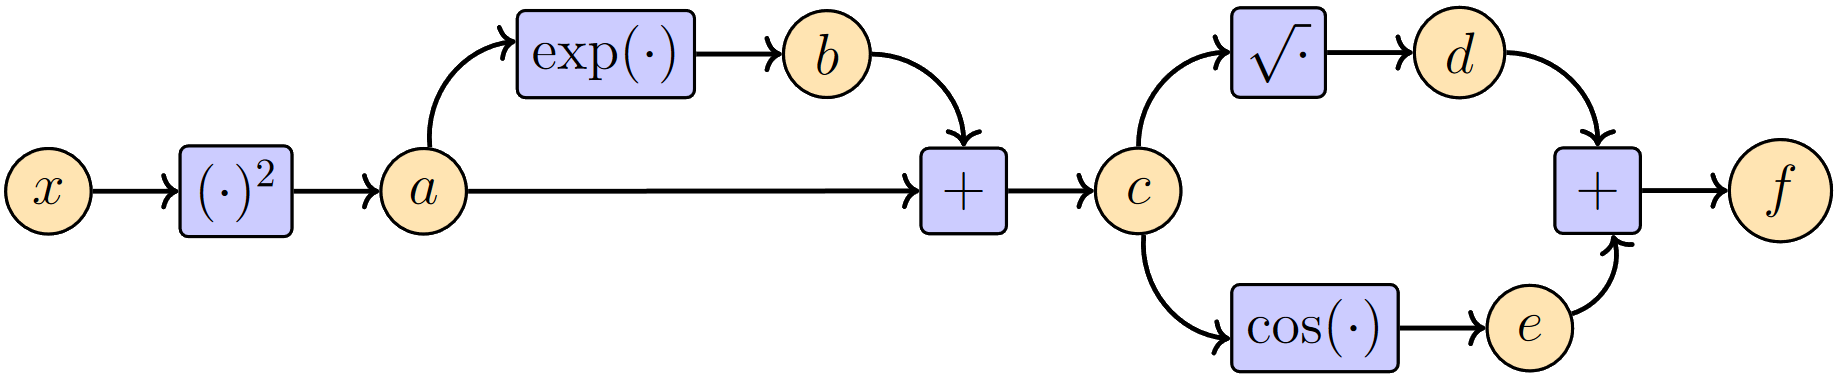
\includegraphics[width=0.75\textwidth]{img/auto_diff.png}
    \end{center}

    We can then compute the derivatives of the intermediate variables w.r.t. their inputs (i.e. inbound edges):\\
    \begin{minipage}{.5\linewidth}
        \[
            \begin{split}
                \frac{\partial a}{\partial x} &= 2x                     \\
                \frac{\partial b}{\partial a} &= \exp(a)                \\
                \frac{\partial c}{\partial a} &= 1                      \\
                \frac{\partial c}{\partial b} &= 1
            \end{split}
        \]
    \end{minipage}%
    \begin{minipage}{.5\linewidth}
        \[
            \begin{split}
                \frac{\partial d}{\partial c} &= \frac{1}{2\sqrt{c}}    \\
                \frac{\partial e}{\partial c} &= -\sin(c)               \\
                \frac{\partial f}{\partial d} &= 1                      \\
                \frac{\partial f}{\partial e} &= 1                      
            \end{split}
        \]
    \end{minipage}\\

    Finally, we can compute $\frac{\partial f}{\partial x}$ by going backward from the output ($f$) to the input ($x$):\\
    \begin{minipage}{.5\linewidth}
        \[
            \begin{split}
                \frac{\partial f}{\partial d} &= \text{ known (previous step)} \\
                \frac{\partial f}{\partial e} &= \text{ known (previous step)} \\
                \frac{\partial f}{\partial c} &= 
                    \frac{\partial f}{\partial d}\frac{\partial d}{\partial c} + \frac{\partial f}{\partial e}\frac{\partial e}{\partial c} \\
            \end{split}
        \]
    \end{minipage}%
    \begin{minipage}{.5\linewidth}
        \[
            \begin{split}
                \frac{\partial f}{\partial b} &= \frac{\partial f}{\partial c}\frac{\partial c}{\partial b} \\
                \frac{\partial f}{\partial a} &= 
                    \frac{\partial f}{\partial b}\frac{\partial b}{\partial a} + \frac{\partial f}{\partial c}\frac{\partial c}{\partial a} \\
                \frac{\partial f}{\partial x} &= \frac{\partial f}{\partial a}\frac{\partial a}{\partial x}                    
            \end{split}
        \]
    \end{minipage}\\

    In other words, to compute the partial derivative of $f$ w.r.t. a variable $x_i$, 
    all variables $w_j$ that follows $x_i$ in the graph are considered.

    Now, by substituting we obtain:
    \[
        \begin{split}
        \frac{\partial f}{\partial c} &= 1 \cdot \frac{1}{2\sqrt{c}} + 1 \cdot (-\sin(c)) \\
        \frac{\partial f}{\partial b} &= \frac{\partial f}{\partial c} \cdot 1 \\
        \frac{\partial f}{\partial a} &= \frac{\partial f}{\partial b} \cdot \exp(a) + \frac{\partial f}{\partial c} \cdot 1 \\
        \frac{\partial f}{\partial x} &= \frac{\partial f}{\partial a} \cdot 2x
        \end{split}
    \] 
\end{example}